Como definido no Capítulo \ref{chap:introducao}, um quadricóptero é uma aeronave cuja propulsão é obtida a partir do uso de quatro rotores e um diagrama o representando é mostrado na Figura \ref{fig:drone_diagram}. 

%\begin{figure}[!htb]
%    \centering
%    \caption{Diagrama de um quadrotor}
%    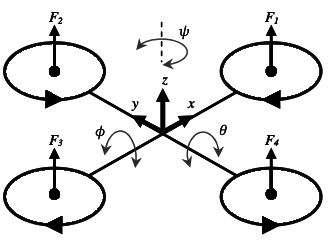
\includegraphics[width=0.6\textwidth]{./04-figuras/drone_diagram/drone_gray_separate1_white}
%    \fonte{Adaptado de \citeonline[p.~1]{Ariffanan2014}}
%    \label{fig:drone_diagram}
%\end{figure}

\begin{figure}[!htb]
    \centering
    \caption{Representação de um quadricóptero}
%    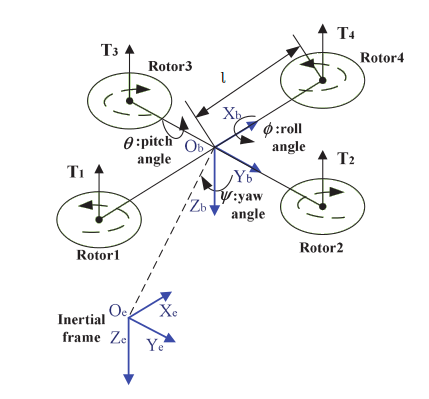
\includegraphics[width=0.6\textwidth]{./04-figuras/drone_diagram/drone_ref19_black_white}
    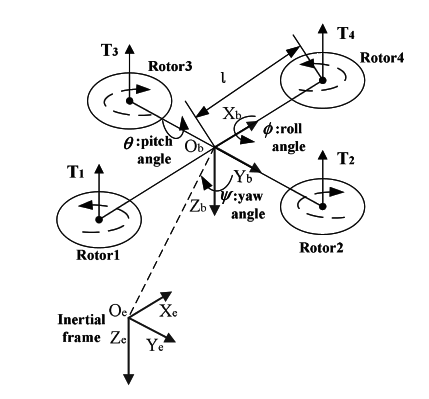
\includegraphics[width=0.7\textwidth]{./04-figuras/drone_diagram/drone_test_sep-1}
    \fonte{Adaptado de \citeonline{Gao2014Stability}}
    \label{fig:drone_diagram}
\end{figure}

Neste diagrama, $x$, $y$ e $z$ indicam a orientação dos eixos, $F_1$, $F_2$, $F_3$ e $F_4$ são as forças geradas pela propulsão de cada um dos motores. As variáveis $\phi$, $\theta$, e $\psi$ são os ângulos de rotação do quadricóptero em relação aos eixos $x$, $y$ e $z$ respectivamente. Estes ângulos são também chamados ângulos de \textit{roll} (rolamento), \textit{pitch} (arfagem) e \textit{yaw} (guinada), respectivamente. Além disto, o diagrama mostra ainda o sentido de rotação de cada um dos quatro rotores. Como se pode ver, os rotores dispostos sobre um mesmo eixo possuem um mesmo sentido de rotação. Desta forma, os rotores 1 e 3 (dispostos sobre o eixo $x$), giram no sentido horário. Já os rotores 2 e 4 (dispostos sobre o eixo $y$) giram no sentido anti-horário. Esta disposição dos rotores permite que os empuxos horizontais se anulem, possibilitando a estabilidade do quadricóptero quando submetido a uma ação de controle devida \cite[p.~1]{Ariffanan2014}.

A estabilidade de um quadricóptero, entretanto, assume mais de uma forma, sendo dividida em dois aspectos principais: altitude e atitude. O primeiro diz respeito ao posicionamento do quadricóptero sobre o eixo $z$ e seu controle é necessário tanto para possibilitar que ele se mantenha num estado estacionário quanto para fazer movimentações no plano XY numa altitude fixa, o que pode ser crucial se ele estiver sendo operado num ambiente limitado inferior e/ou superiormente por alguma espécie de barreira. Já o segundo aspecto, a atitude, se refere à estabilidade angular do quadricóptero, permitindo que sua orientação, representada pelos ângulos $\phi$, $\theta$, e $\psi$ seja controlada.

Uma vez descrito o comportamento geral do sistema, pode-se partir para a sua modelagem matemática. A modelagem retratada é a que foi desenvolvida por \citeonline{Balas2007} e é representada na Figura \ref{fig:diagrama-quadrotor-balas}

\begin{figure}[!htb]
    \centering
    \caption{Diagrama do sistema representando um quadrotor modelado por \citeonline{Balas2007}}
    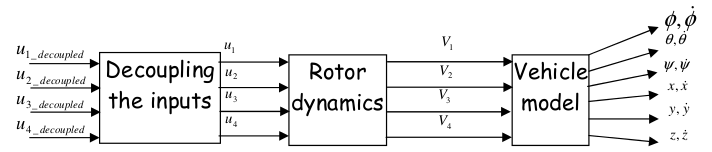
\includegraphics[width=1\textwidth]{./04-figuras/sistemas-nao-lineares/diagrama-quadrotor}
    \fonte{\citeonline[p.~49]{Balas2007}}
    \label{fig:diagrama-quadrotor-balas}
\end{figure}

\section{Modelagem Matemática}
\label{sec:dinamica-rotores}

O quadricóptero é controlado a partir da variação da velocidade dos seus quatro rotores, que são completamente independentes entre si. Desta forma, sendo $l$ o comprimento de cada haste a partir do centro geométrico do quadricóptero e considerando $v_i$ e $\tau_i$ respectivamente como o torque e o impulso do \textit{i}-ésimo rotor, podem-se considerar as entradas do sistema como sendo \cite[p.~4]{Balas2007}:
\begin{align}
u_1 &= \tau_1+\tau_2+\tau_3+\tau_4 \\
u_2 &= l(\tau_3-\tau_4) \\
u_3 &= l(\tau_1-\tau_2) \\
u_4 &= v_1+v_2+v_3+v_4
\end{align}
em que $u_1$ é o impulso total, $u_2$ é o momento de rolamento, $u_3$ é o momento de arfagem e $u_4$ é o momento de guinada.

Além disso, a aceleração em cada eixo pode ser representada por \cite[p.~5]{Balas2007}:
\begin{align}
\ddot{x} &= -\frac{sen(\theta)cos(\phi)}{m}u_1  \\
\ddot{y} &= \frac{sen(\phi)}{m}u_1  \\
\ddot{z} &= - \frac{cos(\theta)cos(\phi)}{m}u_1 +g
\end{align}
em que $\phi$ e $\theta$ são os ângulos em torno dos eixos $x$ e $y$ respectivamente, $m$ é a massa do quadricóptero e $g$ é a gravidade à qual ele é submetido.

Além das acelerações em cada eixo, é também necessário se definir a aceleração \textit{em torno} de cada eixo, ou seja, as acelerações angulares em torno de $x$, $y$ e $z$. Para tanto, assumindo que a estrutura do quadricóptero seja rígida, sendo $I_{xx}$, $I_{yy}$ e $I_{zz}$ o momento de inércia do quadricóptero ao longo dos eixos $x$, $y$ e $z$ respectivamente e considerando que os momentos de inércia ao longo de $x$ e $y$ se equivalem, as acelerações angulares podem ser representadas a partir das seguintes equações \cite[p.~6]{Balas2007}:
\begin{align}
\ddot{\phi} = -\dot{\psi}\dot{\theta}cos(\phi) + 
\frac{cos(\psi)}{I_{xx}}u_2 - 
\frac{sen(\psi)}{I_{yy}}u_3 + 
\frac{I_{yy}-I_{zz}}{I_{xx}}(\dot{\psi}-\dot{\theta}sen(\phi))\dot{\theta}cos(\phi)
\end{align}

\begin{align}
\begin{split}
\ddot{\theta} = \frac{\dot{\psi}\dot{\phi}}{cos(\phi)} +
\dot{\phi}\dot{\theta}tan(\phi) + 
\frac{sen(\psi)}{cos(\phi)I_{xx}}u_2 &+ 
\frac{cos(\psi)}{cos(\phi)I_{yy}}u_3 \\ 
&-\frac{I_{yy}-I_{zz}}{I_{xx}}(\psi-\dot{\theta}sen(\phi))\frac{\dot{\phi}}{cos(\phi)}
\end{split}
\end{align}

\begin{align}
\begin{split}
\ddot{\psi} = \dot{\phi}\dot{\psi}tan(\phi) +
\frac{\dot{\phi}\dot{\theta}}{cos(\phi)} + 
\frac{sen(\psi)tan(\phi)}{I_{xx}}u_2 &+ 
\frac{cos(\phi)tan(\psi)}{I_{yy}}u_3 + 
\frac{1}{I_{zz}}u_4 \\
&-\frac{I_{yy}I_{zz}}{I_{xx}} 
(\dot{\psi}-\dot{\theta}sen(\phi))\dot{\phi}tan(\phi)
\end{split}
\end{align}

Por fim, deve-se relacionar a velocidade de cada rotor \textit{i} ao impulso e torque sobre ele. Esta relação é dada por \cite[p.~7]{Balas2007}:
\begin{equation}
v_i = \tau_i(V_c+v_i)+0.125\rho bcR_p^4\omega_{m\textunderscore i}^2C_d
\end{equation}
sendo $v_i$ o torque sobre o rotor, $\tau_i$ o impulso atuando sobre ele, $V_c$ a velocidade vertical\footnote{A velocidade vertical do quadricóptero também é indicada por $\dot{z}$}, $v_i$ a velocidade induzida no motor, $\rho$ a densidade do ar, $b$ o número de pás, $c$ o comprimento delas, $R_p$ o raio da hélice, $C_d$ o coeficiente de arrasto e $\omega_{m\textunderscore i}$ a velocidade angular do rotor.

Após a modelagem de um sistema complexo como este, é de se desejar que se possa isolar a resposta de determinadas variáveis às entradas. Para tanto, pode-se utilizar o processo de desacoplamento de entradas.


\section{Desacoplamento das Entradas}
\label{sec:desacoplamento}

Para obter uma resposta isolada das variáveis do sistema a partir dos sinais de entrada dele, um bloco de desacoplamento foi modelado em \cite[p.~62]{Balas2007}. Neste caso, foram considerados os acoplamentos entre $\phi$, $\theta$, $\psi$ e $u_2$, $u_3$, $u_4$, relacionados da seguinte maneira:
\begin{align}
u_{2_{\textunderscore decoupled}} &= cos(\psi_{0})u_2 - \frac{I_{xx}sen(\psi_{0})}{I_{yy}}u_3 = I_{xx}\ddot{\phi} \\
u_{3_{\textunderscore decoupled}} &= \frac{sen(\psi_{0})I_{yy}}{cos(\phi_{0})I_{xx}}u_2 + \frac{cos(\psi_{0})}{cos(\phi_{0})}u_3 = I_{yy}\ddot{\theta} \\
u_{4_{\textunderscore decoupled}} &= \frac{I_{zz}sen(\psi_0)tan(\phi_0)}{I_{xx}}u_2 + \frac{I_{zz}cos(\psi_0)tan(\phi_0)}{I_{zz}}u_3 + u_4 = I_{zz}\ddot{\psi} 
\end{align}
em que $\dot{\phi_0}$, $\dot{\theta_0}$ e $\dot{\psi_0}$ são os ângulos no iniciais de rolamento, arfagem e guinada respectivamente; $\dot{\phi}$, $\dot{\theta}$ e $\dot{\psi}$ são os ângulos atuais de rolamento, arfagem e guinada; e $I_{xx}$, $I_{yy}$ e $I_{zz}$ são o momento de inércia em torno dos eixos \textit{x}, \textit{y} e \textit{z} respectivamente.

Como se pode ver pelas equações, aplicando esse desacoplamento obtêm-se as variáveis $u_{2_{\textunderscore decoupled}}$, $u_{3_{\textunderscore decoupled}}$ e $u_{4_{\textunderscore decoupled}}$ relacionadas aos ângulos $\phi$, $\theta$ e $\psi$ respectivamente e considerando o momento de inércia sobre os respectivos eixos, isolando assim a resposta das diferentes variáveis do sistema.

Além disso, a partir destas equações, podem-se representar essas transformações utilizando o formato matricial da seguinte maneira \cite[p.~62]{Balas2007}:
%Nesta estrutura, $u_1$ representa o empuxo total sobre o quadricóptero, $u_2$ representa o momento de \textit{roll} (em torno do eixo $x$), $u_3$ representa o momento de \textit{pitch} (em torno do eixo $y$) e $u_4$ representa o momento de \textit{yaw} (em torno do eixo $z$). $u_{2\textunderscore decoupled}$, $u_{3\textunderscore decoupled}$ e $u_{4\textunderscore decoupled}$ são combinações de $u_2$, $u_3$ e $u_4$ de tal forma que as entradas $u_{2\textunderscore decoupled}$, $u_{3\textunderscore decoupled}$ e $u_{4\textunderscore decoupled}$ tenham as mesmas direções que os ângulos de Euler, $\phi$, $\theta$ e $\psi$, respectivamente. A relação entre estas entradas é dada, em \cite[p.~49]{Balas2007} por:
\[
	\begin{bmatrix}
		u_{2} \\
		u_{3} \\
		u_{4}
	\end{bmatrix} = 
	\begin{bmatrix}
		cos(\psi_0) & sen(\psi_0)cos_(\phi_0)\frac{I_{xx}}{I_{yy}} & 
		0 \\
		
		-sen(\psi_{0})\frac{I_{yy}}{I_{xx}} &
		cos(\psi_{0})cos(\phi_{0}) &
		0 \\
		
		0 &
		-sen(\phi_{0})\frac{I_{zz}}{I_{yy}} &
		1
	\end{bmatrix}
	\begin{bmatrix}
		u_{2\textunderscore decoupled} \\
		u_{3\textunderscore decoupled} \\
		u_{4\textunderscore decoupled}
	\end{bmatrix}
\]

Após os processos de modelagem matemática do sistema e o devido desacoplamento de suas entradas, pode-se representar seu comportamento geral a partir dos espaços de estados, prática comum para descrever sistemas dinâmicos.
%$I_{xx}$, $I_{yy}$ e $I_{zz}$ representam o momento de inércia do quadricóptero ao longo dos eixos $x$, $y$ e $z$, respectivamente.

%\subsection{Funções de Transferência}
%\label{subsec:quadrotor-tfs}
%
%A partir da modelagem feita e já aplicando o desacoplamento implementado, o comportamento geral do quadrotor pode ser representado a partir de três funções de transferência distintas: uma sendo referente ao empuxo vertical; uma segunda, aos momentos de \textit{roll} e \textit{pitch}; e uma terceira, ao momento de \textit{yaw}.

Para se chegar a essas funções de transferência, o primeiro aspecto a ser considerado é que a relação entre a tensão e o torque é dado por uma aproximação feita a partir de \cite[p.~25]{Balas2007}:
\begin{equation}
H(s)=\frac{K}{1+\tau s}
\end{equation}
em que $\tau$ é uma constante de tempo $\tau = 0,314$ e que $K$ é o ganho CC do rotor definido como $K=0.045$N.m/V para exemplificar o sistema.

Desta forma, tem-se:
\begin{equation}
\frac{u_4}{V_1-V_2+V_3-V_4} = \frac{0,045}{0,314s + 1}
\end{equation}

%Assumindo um quadricóptero com massa $m$ igual a 2,354 g e uma aceleração $g$ igual a 9,81 N.
A partir dessas relações, a função de transferência obtida por \citeonline[p.~35]{Balas2007} para representar o empuxo vertical gerado pelos quatro rotores do quadrotor foi:
\begin{equation}
H(s) = \frac{u_1}{V_1+V_2+V_3-V_4} = \frac{2,105s-0,0425}{0,4895s^2+1,873s+1} N/V
\end{equation}

Já a função de transferência obtida para representar os momentos de \textit{roll} e de \textit{pitch} foi \cite[p.~35]{Balas2007}:
\begin{equation}
H(s) = \frac{u_2}{V_4-V_2} = \frac{u_3}{V_1-V_3} = l\frac{1,155s}{0,8696s^2+0,401s+1} Nm/V
\end{equation}

Por fim, a função de transferência obtida para representar o momento de \textit{yaw} foi \cite[p.~35]{Balas2007}:
\begin{equation}
H(s) =  \frac{u_4}{V_1-V_2+V_3-V_4} = \frac{0,045}{0,314s+1} Nm/V
\end{equation}

Uma forma alternativa à representação por funções de transferência é a representação no espaço de estados, que é mostrada na seção a seguir.


\subsection{Representação no Espaço de Estados}
\label{subsec:quadrotor-ss}

Como mostrado em \cite[p.~63]{Balas2007}, o sistema modelado, já incluindo o desacoplamento de entradas, pode ser representado da seguinte forma no espaço de estados.
\begin{align} \label{eq:space_state_equation_quadcopter}
	\dot{x} &= Ax + Bu \nonumber \\
	y		&= Cx + Du
\end{align}

Com o vetor de estados $X$ sendo dado por:
\begin{equation*}
X=
\left[ \begin{array}{@{}*{12}{c}@{}}
     x & y & z & \dot{x} & \dot{y} & \dot{z} & \phi & \theta & \psi & \dot{\phi} & \dot{\theta} & \dot{\psi}\\
\end{array} \right]^T
\end{equation*}

O vetor de entrada $U$ sendo:
\[ 
	U =
	\begin{bmatrix}
		u_1 & 
		u_{2\textunderscore decoupled} &
		u_{3\textunderscore decoupled} &
		u_{4\textunderscore decoupled}
	\end{bmatrix}^T
\]

E as matrizes A, B, C e D sendo definidas como:
\begin{equation*}
A =
\left[ \begin{array}{@{}*{12}{c}@{}}
     0 & 0 & 0 & 1 & 0 & 0 & 0 & 0  & 0 & 0 & 0 & 0 \\
     0 & 0 & 0 & 0 & 1 & 0 & 0 & 0  & 0 & 0 & 0 & 0 \\
     0 & 0 & 0 & 0 & 0 & 1 & 0 & 0  & 0 & 0 & 0 & 0 \\
     0 & 0 & 0 & 0 & 0 & 0 & 0 & -g & 0 & 0 & 0 & 0 \\
     0 & 0 & 0 & 0 & 0 & 0 & g & 0  & 0 & 0 & 0 & 0 \\
     0 & 0 & 0 & 0 & 0 & 0 & 0 & 0  & 0 & 0 & 0 & 0 \\
     0 & 0 & 0 & 0 & 0 & 0 & 0 & 0  & 0 & 1 & 0 & 0 \\
     0 & 0 & 0 & 0 & 0 & 0 & 0 & 0  & 0 & 0 & 1 & 0 \\
     0 & 0 & 0 & 0 & 0 & 0 & 0 & 0  & 0 & 0 & 0 & 1 \\
     0 & 0 & 0 & 0 & 0 & 0 & 0 & 0  & 0 & 0 & 0 & 0 \\
     0 & 0 & 0 & 0 & 0 & 0 & 0 & 0  & 0 & 0 & 0 & 0 \\
     0 & 0 & 0 & 0 & 0 & 0 & 0 & 0  & 0 & 0 & 0 & 0 \\
\end{array}\right]
\end{equation*}

\begin{equation*}
B =
\left[\begin{array}{@{}*{4}{c}@{}}
	0 & 0 & 0 & 0 \\
	0 & 0 & 0 & 0 \\
	0 & 0 & 0 & 0 \\
	0 & 0 & 0 & 0 \\
	0 & 0 & 0 & 0 \\
	-1/m & 0 & 0 & 0 \\
	0 & 0 & 0 & 0 \\
	0 & 0 & 0 & 0 \\
	0 & 0 & 0 & 0 \\
	0 & cos(\psi_0)/I_{xx} & -sen(\psi_0)/I_{yy} & 0 \\
	0 & sen(\psi_0)/(cos(\phi_0)I_{xx}) & cos(\psi_0)/(cos(\phi_0)I_{yy}) & 0\\
	0 & sin(\psi_0)tan(\phi_0)/I_{xx} & cos(\psi_0)
	tan(\phi_0)/I_{yy} & 1/I_{zz} \\
\end{array}\right]
\end{equation*}

\begin{equation*}
C =
\left[ \begin{array}{@{}*{12}{c}@{}}
	1 & 0 & 0 & 0 & 0 & 0 & 0 & 0 & 0 & 0 & 0 & 0 \\
	0 & 1 & 0 & 0 & 0 & 0 & 0 & 0 & 0 & 0 & 0 & 0 \\
	0 & 0 & 1 & 0 & 0 & 0 & 0 & 0 & 0 & 0 & 0 & 0 \\
	0 & 0 & 0 & 1 & 0 & 0 & 0 & 0 & 0 & 0 & 0 & 0 \\
	0 & 0 & 0 & 0 & 1 & 0 & 0 & 0 & 0 & 0 & 0 & 0 \\
	0 & 0 & 0 & 0 & 0 & 1 & 0 & 0 & 0 & 0 & 0 & 0 \\
	0 & 0 & 0 & 0 & 0 & 0 & 1 & 0 & 0 & 0 & 0 & 0 \\
	0 & 0 & 0 & 0 & 0 & 0 & 0 & 1 & 0 & 0 & 0 & 0 \\
	0 & 0 & 0 & 0 & 0 & 0 & 0 & 0 & 1 & 0 & 0 & 0 \\
	0 & 0 & 0 & 0 & 0 & 0 & 0 & 0 & 0 & 1 & 0 & 0 \\
	0 & 0 & 0 & 0 & 0 & 0 & 0 & 0 & 0 & 0 & 1 & 0 \\
	0 & 0 & 0 & 0 & 0 & 0 & 0 & 0 & 0 & 0 & 0 & 1 \\
\end{array}\right]
\end{equation*}

\begin{equation*}
D =
\left[\begin{array}{@{}*{4}{c}@{}}
	0 & 0 & 0 & 0 \\
	0 & 0 & 0 & 0 \\
	0 & 0 & 0 & 0 \\
	0 & 0 & 0 & 0 \\
	0 & 0 & 0 & 0 \\
	0 & 0 & 0 & 0 \\
	0 & 0 & 0 & 0 \\
	0 & 0 & 0 & 0 \\
	0 & 0 & 0 & 0 \\
	0 & 0 & 0 & 0 \\
	0 & 0 & 0 & 0 \\
	0 & 0 & 0 & 0 \\
\end{array}\right]
\end{equation*}
em que $g$ é a gravidade, $m$, a massa do quadricóptero e os ângulos $\phi_0$, $\theta_0$ e $\psi_0$ representam os ângulos iniciais em torno dos eixos $x$, $y$ e $z$ respectivamente. Além disto, $I_{xx}$, $I_{yy}$ e $I_{zz}$ representam o momento de inércia do quadricóptero ao longo destes mesmos eixos.

Como se pode perceber, a matriz C é uma matriz diagonal, o que implica no fato de a saída do sistema ser representada pelo vetor de estados.

Ao longo deste trabalho, essa foi a modelagem adotada para simular o sistema de um quadricóptero.
